
%%% Local Variables:
%%% mode: latex
%%% TeX-master: t
%%% End:

\chapter{原理分析}
\label{cha:intro}

\section{震源基础}
1906年旧金山发生了一次在地震学上具有重在研究意义的地震,地震前后对圣安德烈亚斯断层的研究结果\citep{Milne1910}使人们普遍认为发生地震的原因是震源处的断层发生了滑移错动,巨大的势能转化为了热能及地震波等能力。这种错动可由位错理论进行解释,位错理论认为地震的发生是因为应力长期缓慢的大量积累,最终达到了断层锁定的极限,引发断层面(原有断层或地震新生断层)两侧发生突然的位错,导致了应力释放并形成地震。自此以后,对于地震震源的研究就开始集中到断层面的研究上。通常认为断层面两侧的应力在地震发生前后都是连续的,只有位移在断层面两侧突然间断,所以研究清楚断层面上的所有运动学信息是研究整个震源过程的主要内容。如果进一步简化,将地震发生时断层的位错视为纯剪切的点源位错(事实证明该简化很多情况下是合理的,且本文只讨论该情况),则利用三个描述断层的参数便可完整描述震源的物理过程(不考虑时间函数),并称该三参数为震源的机制解。求解震源机制的过程便是求解该三个参数的过程,该三参数具体定义如图\ref{fig01}所示\citep{程万正2006}。
\begin{figure}
\centering
%  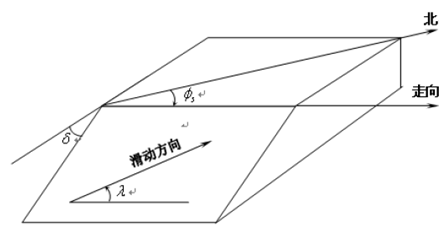
\includegraphics[width=\textwidth]{fig01.png} 
  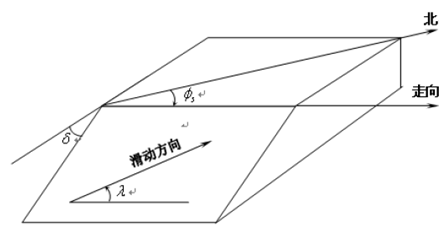
\includegraphics{fig01.png} 
  \caption{震源机制三个参数的具体意义}
  \label{fig01}
\end{figure}

\section{反演方法}
\subsection{波形分解}
理论研究表明,同步地震点源\citep{Silver1982}所激发的地震波场如公式\ref{eq01}\citep{Jost1989}。
\begin{equation}
\label{eq01}
d_n(x,t)=M_{ki}[G_{nk,i}*s(t)]
\end{equation}

其中$s(t)$为震源时间函数,$Mkj$为地震矩张量,$G_{nk,i}$为格林函数,从上式可知理论波形$d$与$Mi$为线性关系。根据\citet{Kikuchi1991}的分解方法,任意地震矩张量均可由6个简单地震矩张量通过线性组合而成,如公式\ref{eq02}。
\begin{equation}
\label{eq02}
M=\sum_{k=1}^6a_kM_k
\end{equation}

公式\ref{eq02}中等式右边的$M_k$如公式\ref{eq03}所示。
\begin{equation}
\label{eq03}
\begin{array}{ccc}
M_1=\left[\begin{array}{ccc}
0 & 1 & 0\\
1 & 0 & 0\\
0 & 0 & 0\\
\end{array}\right]&
M_2=\left[\begin{array}{ccc}
1 & 0 & 0\\
0 & -1 & 0\\
0 & 0 & 0\\
\end{array}\right]&
M_3=\left[\begin{array}{ccc}
0 & 0 & 0\\
0 & 0 & 1\\
0 & 1 & 0\\
\end{array}\right]\\
M_4=\left[\begin{array}{ccc}
0 & 0 & 1\\
0 & 0 & 0\\
1 & 0 & 0\\
\end{array}\right]&
M_5=\left[\begin{array}{ccc}
-1 & 0 & 0\\
0 & 0 & 0\\
0 & 0 & 1\\
\end{array}\right]&
M_6=\left[\begin{array}{ccc}
1 & 0 & 0\\
0 & 1 & 0\\
0 & 0 & 1\\
\end{array}\right]\\
\end{array}
\end{equation}

$M_1$-$M_6$为6个简单的地震源,其中$M_6$代表爆炸源,其余5个均为剪切位错源,根据公式\ref{eq02}和公式\ref{eq03}推导可知系数a与M各分量间的对应关系如公式\ref{eq04}和公式\ref{eq05}。
\begin{equation}
\label{eq04}
M=\left[\begin{array}{ccc}
a_2-a_5+a_6 & a_1 & a_4\\
a_1 & -a_2+a_6 & a_3\\
a_4 & a_3 & a_5+a_6\\
\end{array}\right]\\
\end{equation}

\begin{equation}
\label{eq05}
\left[\begin{array}{c}
a_1\\
a_2\\
a_3\\
a_4\\
a_5\\
a_6\\
\end{array}\right]=
\left[\begin{array}{c}
M_{12}\\
(M_{11}+M_{33}-2M_{22})/3\\
M_{23}\\
M_{13}\\
(2M_{33}-M_{11}-M_{22})/3\\
(M_{11}+M_{22}+M_{33})/3\\
\end{array}\right]
\end{equation}

将公式\ref{eq02}代入公式\ref{eq01},并省略波形分量指标$n$可得到公式\ref{eq06}。
\begin{equation}
\label{eq06}
d=\sum_{k=1}^{6}a_kd_k
\end{equation}

再将公式\ref{eq05}所示的$a$与$M$关系代入公式\ref{eq06}可得到$d$关于$M$与$d_k$的公式\ref{eq07}。
\begin{equation}
\label{eq07}
\begin{array}{rl}\\
d=&M_{11}(1/3d_2-1/3d_5+1/3d_6)+M_{12}d_1+M_{13}d_4\\
&+M_{22}(-2/3d_2-1/3d_5+1/3d_6)+M_{23}d_3\\
&+M_{33}(1/3d_2+2/3d_5+1/3d_6))
\end{array}
\end{equation}

为进一步简化,将公式\ref{eq07}中$M$矩阵的6个分量依次记为 $M_1,M_2,M_3,M_4,M_5,M_6$,并将与$Mi$相乘的关于$d_k$的多项式简记为$G_i$,于是得到了简洁的6项求和的理论波形公式\ref{eq08}。在此我们按照\citet{Stein2003}专著中关于地震矩反演章节中对格林函数的推广定义,将公式\ref{eq08}中的$G_i$也称为格林函数,此格林函数即是我们之后在CPS反演中需要用到的。
\begin{equation}
\label{eq08}
d=G_iM_i(i=1,2,...6)
\end{equation}

于是任意地震矩产生的波形均可由其矩张量矩阵和6个格林函数线性叠加得到,而格林函数又可由6个已知基本地震矩激发的波形$d_k(k=1,2,...6)$叠加得到。由于以上运算均是线性运算,在$d_k$已知的情况下,在计算机中经两次迭加得到$d$速度非常快。

至此,我们已经将任意剪切位错源的波形分解为6个基本震源波形的线性叠加,而叠加的系数可由该位错源的震源机制唯一确定。现在的关键问题转化为计算6个基本震源对应的理论波形$d_k$,这可通过之后要介绍的格林函数库快速实现。

\subsection{格林函数库}

通常情况下天然地震由断层间错动造成,震源均近似纯剪切位错源。习惯上人们用破裂断层的三个角度参数——走向,倾角和滑动角来更直观地描述震源机制,地震矩张量与震源机制三个参数的对应关系如公式\ref{eq09}所示\citep{Aki1980}。
\begin{equation}
\label{eq09}
\left\{
    \begin{array}{l}
    M_{11}=-M_0(sin{\delta}cos{\lambda}sin{2\phi_s}+sin{2\delta}sin{\lambda}sin^2{\phi_s})\\
    M_{12}=M_0(sin{\delta}cos{\lambda}cos{2\phi_s}+1/2sin{2\delta}sin{\lambda}sin{2\phi_s})\\
    M_{13}=-M_0(cos{\delta}cos{\lambda}cos{\phi_s}+cos{2\delta}sin{\lambda}sin{\phi_s})\\
    M_{22}=M_0(sin{\delta}cos{\lambda}cos{2\phi_s}-sin{2\delta}sin{\lambda}cos^2{\phi_s})\\
    M_{23}=-M_0(cos{\delta}cos{\lambda}sin{\phi_s}-cos{2\delta}sin{\lambda}cos^2{\phi_s})\\
    M_{33}=M_0sin{2\delta}sin{\lambda}\\
    \end{array}
\right.
\end{equation}

其中,$\phi_s$是走向,$\delta$是倾角,$lambda$是滑动角。 $M_0$是最早由\citet{Aki1966}提出的用来度量震源长周期辐射的强度,最初称为地震矩。由于是一个标量,现在又叫作标量地震矩,代表了地震的强度。将公式\ref{eq09}代入公式\ref{eq08}即将公式转化为了理论波形关于震源机制三参数的形式。

现在我们进一步研究$d_k$如何计算,在均匀介质\citep{Ben-Menahem1963}和层状介质\citep{Haskell1964}模型的面波波场辐射理论基础上,\citet{Wang1980} 进一步得到了剪切位错源在层状速度模型中所激发的地震波场,在柱坐标频域下的表示,如公式\ref{eq10}所示。
\begin{equation}
\label{eq10}
\left\{
    \begin{array}{l}
    U_z(r,\phi,0,\omega)=Z_{SS}{\cdot}s_2+Z_{DS}{\cdot}s_3+Z_{DD}{\cdot}s_1\\
    U_r(r,\phi,0,\omega)=R_{SS}{\cdot}s_2+R_{DS}{\cdot}s_3+R_{DD}{\cdot}s_1\\
    U_{\phi}(r,\phi,0,\omega)=T_{SS}{\cdot}t_2+T_{DS}{\cdot}t_1\\
    \end{array}
\right.
\end{equation}

公式\ref{eq10}中各符号意义如\ref{eq11}所示,\ref{eq11}中$\phi$是地震观测台站相对震源的方位角,$\lambda$,$\delta$,${\phi}_s$分别代表断层滑动角,倾角,走向。公式\ref{eq10}中的$Z_{SS}$,$R_{SS}$,$T_{SS}$分别对应于$\delta=90^\circ$,$\lambda=0^\circ$的纯走滑型断裂的理论地震图的垂向、径向、切向分量;$Z_{DS}$,$R_{DS}$,$T_{DS}$分别代表$lambda=90^\circ$,$\delta=90^\circ$的纯倾滑型逆冲断层激发的地震波的垂向、径向、切向分量;$Z_{DD}$和$R_{DD}$分别对应于倾角$\delta=45^\circ$,滑动角$\lambda=90^\circ$的逆冲断层激发的理论地震波的垂向、径向分量。它们8个是合成任意剪切位错源理论地震图所需要的全部基本函数,它们是对波数K的积分表达\citep{Wang1980} 。格林函数库即由大量的不同震中距,不同震源深度对应的这8个基本函数组成。
\begin{equation}
\label{eq11}
\left\{
    \begin{array}{l}
    s_1=1/2{sin\lambda}sin{2\delta}\\
    s_2={cos\lambda}{sin\delta}sin2({\phi}-{\phi}_s)+1/2{sin\lambda}{sin2\delta}cos2({\phi}-{\phi}_s)\\
    s_3=-{cos\lambda}{cos\delta}cos({\phi}-{\phi}_s)+{sin\lambda}{cos2\delta}sin({\phi}-{\phi}_s)\\
    t_1={cos\lambda}{cos\delta}sin({\phi}-{\phi}_s)+{sin\lambda}{cos2\delta}cos({\phi}-{\phi}_s)\\
    t_2={cos\lambda}{sin\delta}cos2({\phi}-{\phi}_s)-1/2{sin\lambda}{sin2\delta}sin2({\phi}-{\phi}_s)\\
    \end{array}
\right.
\end{equation}

利用公式\ref{eq09}可推算出公式\ref{eq03}中所示6个基本地震所对应的震源机制,即各地震的3个角度参数,将其代入公式\ref{eq10},并积分变换到时间域,便得到了$d_k$,进而得到$d$。而根据公式\ref{eq11}知$s_1$、$s_2$、$s_3$、$t_1$、$t_2$等量均与$\omega$无关,结合公式\ref{eq10}可推得时间域的$Z_{SS}$,$R_{DD}$等量与$d_k$的关系也是线性的,可通过快速线性叠加得到。
综上分析知,计算$d$的关键在于得到该速度模型下,对应震中距和震源深度的$Z_{SS}$,$R_{DD}$等基本函数。而计算该函数由于要经过大量积分运算,计算速度非常慢,在迭代或搜索反演过程中实时计算一系列该基本函数是不可取的。在实际工作中通过将研究区域按一定精度格点划分,并事先计算好各格点的基本函数,并将大量的各点所对应的基本函数归档存储为格林函数库。之后理论波形数值计算需要时,直接在格林函数库中调用对应震中距和震源深度的基本函数即可,这样便实现了$d$的快速计算。经检验,这样叠加计算理论波形的速度非常快,能满足格点搜索时大量理论波形图计算的需要。

\subsection{格点搜索}

CAP与CPS方法计算波形的拟合度时使用了不同的目标函数,CAP方法先将理论波形与实测波形通过互相关运算进行时差调整,再计算调整后的波形间残差范数(L1或L2)\citep{Zhao1994},该残差范数定为为最终的目标函数,CPS方法则直接将理论与实测波形的互相关函数作为目标函数。为了单独分析权重因素对反演的影响,对比CPS与CAP不同定权的差异,后文反演试验及讨论均基于CPS的目标函数方案。CPS方法中的互相关目标函数Fit如公式\ref{eq12}定义。
\begin{equation}
\label{eq12}
Fit=(\int_{Tb}^{Te}Y(t)G(t)dt)^2/(\int_{Tb}^{Te}Y(t)Y(t)dt*\int_{Tb}^{Te}G(t)G(t)dt)
\end{equation}

在计算机中进行数值计算时使用公式\ref{eq13}所示离散形式:
\begin{equation}
\label{eq13}
Fit=[\sum_{j=1}^{N}\sum_{m-1}^{6}yg(j,m,k)M_m]^2/{[\sum_{j=1}^{N}yy(j)][\sum_{j=1}^{N}\sum_{m=1}^{6}\sum_{n=1}^{6}gg(j,m,n)M_mM_n]}
\end{equation}

公式\ref{eq13}中各符号表示的含义如公式\ref{eq14}和公式\ref{eq15}所示。
\begin{equation}
\label{eq14}
\left\{
    \begin{aligned}
    yy(j)&=\sum_{h=1}^{H(j)}y(j,h)y(j,h)wt(j)\\
    gg(j,m,n))&=\sum_{h=1}^{H(j)}g_{m}(j,h)g_{n}(j,h)wt(j)\\
    yg(j,m,k))&=\sum_{h=1}^{H(j)-|k|}\mathop{{y}'}(j,h)\mathop{{g}'_{m}}(j,h)wt(j)
    \end{aligned}
\right.
\end{equation}

\begin{equation}
\label{eq15}
\left\{
    \begin{aligned}
    \mathop{{y}'}(j,h)&=y(j,h+k) &k\geq0 \\
    \mathop{{g}'}(j,h)&=g(j,h)   &k\geq0 \\
    \mathop{{y}'}(j,h)&=y(j,h)   &k<0 \\
    \mathop{{g}'}(j,h)&=g(j,h-k) &k<0 \\
    \end{aligned}   \\
\right.
\end{equation}

N为参与反演的观测波形总道数,$H(j),wt(j)$分别为第$j(j=1,2,...N)$道波形的总采样点数及权重因子,$y(j,h),g(j,h)$分别为公式\ref{eq08}中,第$j$道观测波形$d(j)$及其对应的格林函数$Gi(j)$经过相同的数据处理(去噪等),可直接用于反演的波形的第$h(h=1,H)$个采样点,$k$为使$yg(j,m,k)$取得最大值的整数,它是Tan等\citep{Tan2006}提出的到时差平移参数,可以有效地减小系统性误差的影响。本文计算的矩震级$M_w$是由波形振幅比值计算得到的标量矩转换得到的,采用如公式\ref{eq16}所示2005年被CoSOI(Commission on Seismological Observation and Interpretation)采纳的IASPEI标准,其中Mo的单位为dyne-cm。
\begin{equation}
\label{eq16}
	M_w=2/3(logM_0-16.1)
\end{equation}

理论地震图可用多种方法计算,本文通过之前章节所述的用格林函数库快速合成理论波形,而格林函数库则用CPS软件包中的hprep96,hspec96,hpulse96子程序计算得到,该子程序的基本原理是波数积分法。反演时考虑到震源机制解的全空间(走向0°-360°,倾角0°-90°,滑动角-180°-180°)较小,通常采用全空间格点搜索法。
格点搜索法将全空间划分为一定精度间隔的格点,并依次遍历全部格点找寻目标函数最值点,最值处对应格点即为最优解。本文如公式\ref{eq13}所示目标函数Fit的具体计算过程如下,将遍历到的格点震源机制转换为等价地震矩张量\citep{Jost1989},同时用格林函数库快速求出公式\ref{eq08}中对应的格林函数$Gi$,将格林函数$Gi$,观测波形$d$进行必要且相同的滤波、截取时窗处理,并将处理后格林函数$g$,观测波形$y$和地震矩张量$M$与代入公式\ref{eq13},计算即可求得该格点处的拟合度Fit。

\section{定权优化}
\label{sec:first}

苏轼(1037-1101),北宋文学家、书画家。字子瞻,号东坡居士,眉州眉山(今属四川)人
。苏洵子。嘉佑进士。神宗时曾任祠部员外郎,因反对王安石新法而求外职,任杭州通判,
知密州、徐州、湖州。后以作诗“谤讪朝廷”罪贬黄州。哲宗时任翰林学士,曾出知杭州、
颖州等,官至礼部尚书。后又贬谪惠州、儋州。北还后第二年病死常州。南宋时追谥文忠。
与父洵弟辙,合称“三苏”。在政治上属于旧党,但也有改革弊政的要求。其文汪洋恣肆,
明白畅达,为“唐宋八大家”之一。  其诗清新豪健,善用夸张比喻,在艺术表现方面独具
风格。少数诗篇也能反映民间疾苦,指责统治者的奢侈骄纵。词开豪放一派,对后代很有影
响。《念奴娇·赤壁怀古》、《水调歌头·丙辰中秋》传诵甚广。

{\kaishu 坡仙擅长行书、楷书,取法李邕、徐浩、颜真卿、杨凝式,而能自创新意。用笔丰腴
  跌宕,有天真烂漫之趣。与蔡襄、黄庭坚、米芾并称“宋四家”。能画竹,学文同,也喜
  作枯木怪石。论画主张“神似”,认为“论画以形似,见与儿童邻”;高度评价“诗中有
  画,画中有诗”的艺术造诣。诗文有《东坡七集》等。存世书迹有《答谢民师论文帖》、
  《祭黄几道文》、《前赤壁赋》、《黄州寒食诗帖》等。  画迹有《枯木怪石图》、《
  竹石图》等。}

{\fangsong 易与天地准,故能弥纶天地之道。仰以观於天文,俯以察於地理,是故知幽明之故。原
  始反终,故知死生之说。精气为物,游魂为变,是故知鬼神之情状。与天地相似,故不违。
  知周乎万物,而道济天下,故不过。旁行而不流,乐天知命,故不忧。安土敦乎仁,故
  能爱。范围天地之化而不过,曲成万物而不遗,通乎昼夜之道而知,故神无方而易无体。}

% 非本科生一般用不到幼圆与隶书字体。需要的同学可以使用 thufonts.def 文件
% 自行配置中文字体,或者换用 pdflatex 引擎编译。
{\ifcsname youyuan\endcsname\youyuan 有天地,然后万物生焉。盈天地之间者,唯万物,故受之以屯;屯者盈也,屯者物之
  始生也。物生必蒙,故受之以蒙;蒙者蒙也,物之穉也。物穉不可不养也,故受之以需;
  需者饮食之道也。饮食必有讼,故受之以讼。讼必有众起,故受之以师;师者众也。众必
  有所比,故受之以比;比者比也。比必有所畜也,故受之以小畜。物畜然后有礼,故受之
  以履。\fi}

{\heiti 履而泰,然后安,故受之以泰;泰者通也。物不可以终通,故受之以否。物不可以终
  否,故受之以同人。与人同者,物必归焉,故受之以大有。有大者不可以盈,故受之以谦。
  有大而能谦,必豫,故受之以豫。豫必有随,故受之以随。以喜随人者,必有事,故受
  之以蛊;蛊者事也。}

{\ifcsname lishu\endcsname\lishu 有事而后可大,故受之以临;临者大也。物大然后可观,故受之以观。可观而后有所合
  ,故受之以噬嗑;嗑者合也。物不可以苟合而已,故受之以贲;贲者饰也。致饰然后亨
  ,则尽矣,故受之以剥;剥者剥也。物不可以终尽,剥穷上反下,故受之以复。复则不
  妄矣,故受之以无妄。\fi}

{\songti 有无妄然后可畜,故受之以大畜。物畜然后可养,故受之以颐;颐者养也。不养则不
  可动,故受之以大过。物不可以终过,故受之以坎;坎者陷也。陷必有所丽,故受之以
  离;离者丽也。}

\section{误差评定}
\label{chap1:sample:table} 

\subsection{基本表格}
\label{sec:basictable}

模板中关于表格的宏包有三个: \textsf{booktabs}、\textsf{array} 和
\textsf{longtabular},命令有一个 \verb|\hlinewd|。三线表可以用 \textsf{booktabs}
提供的 \verb|\toprule|、\verb|\midrule| 和 \verb|\bottomrule|。它们与
\textsf{longtable} 能很好的配合使用。如果表格比较简单的话可以直接用命令
\verb|hlinewd{xpt}| 控制。
\begin{table}[htb]
  \centering
  \begin{minipage}[t]{0.8\linewidth} % 如果想在表格中使用脚注,minipage是个不错的办法
  \caption[模板文件]{模板文件。如果表格的标题很长,那么在表格索引中就会很不美
    观,所以要像 chapter 那样在前面用中括号写一个简短的标题。这个标题会出现在索
    引中。}
  \label{tab:template-files}
    \begin{tabular*}{\linewidth}{lp{10cm}}
      {\heiti 文件名} & {\heiti 描述} \\
      thuthesis.ins & \LaTeX{} 安装文件,docstrip\footnote{表格中的脚注} \\
      thuthesis.dtx & 所有的一切都在这里面\footnote{再来一个}。\\
      thuthesis.cls & 模板类文件。\\
      thuthesis.cfg & 模板配置文。cls 和 cfg 由前两个文件生成。\\
      thubib.bst    & 参考文献 Bibtex 样式文件。\\
      thutils.sty   & 常用的包和命令写在这里,减轻主文件的负担。\\
    \end{tabular*}
  \end{minipage}
\end{table}

首先来看一个最简单的表格。表 \ref{tab:template-files} 列举了本模板主要文件及其功
能。请大家注意三线表中各条线对应的命令。这个例子还展示了如何在表格中正确使用脚注。
由于 \LaTeX{} 本身不支持在表格中使用 \verb|\footnote|,所以我们不得不将表格放在
小页中,而且最好将表格的宽度设置为小页的宽度,这样脚注看起来才更美观。

\subsection{复杂表格}
\label{sec:complicatedtable}

我们经常会在表格下方标注数据来源,或者对表格里面的条目进行解释。前面的脚注是一种
不错的方法,如果你不喜欢脚注。那么完全可以在表格后面自己写注释,比如表~\ref{tab:tabexamp1}。
\begin{table}[htbp]
  \centering
  \caption{复杂表格示例 1}
  \label{tab:tabexamp1}
  \begin{minipage}[t]{0.8\textwidth} 
    \footnotesize 注:数据来源《使用手册》。\\
    *:东部\\
    **:西部
  \end{minipage}
\end{table}

此外,表~\ref{tab:tabexamp1} 同时还演示了另外两个功能:1)通过 \textsf{tabularx} 的
 \texttt{|X|} 扩展实现表格自动放大;2)通过命令 \verb|\diagbox| 在表头部分
插入反斜线。

为了使我们的例子更接近实际情况,我会在必要的时候插入一些“无关”文字,以免太多图
表同时出现,导致排版效果不太理想。第一个出场的当然是我的最爱:风流潇洒、骏马绝尘、
健笔凌云的{\heiti 李太白}了。

李白,字太白,陇西成纪人。凉武昭王暠九世孙。或曰山东人,或曰蜀人。白少有逸才,志
气宏放,飘然有超世之心。初隐岷山,益州长史苏颋见而异之,曰:“是子天才英特,可比
相如。”天宝初,至长安,往见贺知章。知章见其文,叹曰:“子谪仙人也。”言于明皇,
召见金銮殿,奏颂一篇。帝赐食,亲为调羹,有诏供奉翰林。白犹与酒徒饮于市,帝坐沉香
亭子,意有所感,欲得白为乐章,召入,而白已醉。左右以水颒面,稍解,援笔成文,婉丽
精切。帝爱其才,数宴见。白常侍帝,醉,使高力士脱靴。力士素贵,耻之,摘其诗以激杨
贵妃。帝欲官白,妃辄沮止。白自知不为亲近所容,恳求还山。帝赐金放还。乃浪迹江湖,
终日沉饮。永王璘都督江陵,辟为僚佐。璘谋乱,兵败,白坐长流夜郎,会赦得还。族人阳
冰为当涂令,白往依之。代宗立,以左拾遗召,而白已卒。文宗时,诏以白歌诗、裴旻剑舞、
然后就是忧国忧民,诗家楷模杜工部了。杜甫,字子美,其先襄阳人,曾祖依艺为巩令,因
居巩。甫天宝初应进士,不第。后献《三大礼赋》,明皇奇之,召试文章,授京兆府兵曹参
军。安禄山陷京师,肃宗即位灵武,甫自贼中遁赴行在,拜左拾遗。以论救房琯,出为华州
司功参军。关辅饥乱,寓居同州同谷县,身自负薪采梠,餔糒不给。久之,召补京兆府功曹,
道阻不赴。严武镇成都,奏为参谋、检校工部员外郎,赐绯。武与甫世旧,待遇甚厚。乃于
成都浣花里种竹植树,枕江结庐,纵酒啸歌其中。武卒,甫无所依,乃之东蜀就高適。既至
而適卒。是岁,蜀帅相攻杀,蜀大扰。甫携家避乱荆楚,扁舟下峡,未维舟而江陵亦乱。乃
溯沿湘流,游衡山,寓居耒阳。卒年五十九。元和中,归葬偃师首阳山,元稹志其墓。天宝
间,甫与李白齐名,时称李杜。然元稹之言曰:“李白壮浪纵恣,摆去拘束,诚亦差肩子美
矣。至若铺陈终始,排比声韵,大或千言,次犹数百,词气豪迈,而风调清深,属对律切,
而脱弃凡近,则李尚不能历其藩翰,况堂奥乎。”白居易亦云:“杜诗贯穿古今,  尽工尽
善,殆过于李。”元、白之论如此。盖其出处劳佚,喜乐悲愤,好贤恶恶,一见之于诗。而
又以忠君忧国、伤时念乱为本旨。读其诗可以知其世,故当时谓之“诗史”。旧集诗文共六
十卷,今编诗十九卷。

\begin{table}[htbp]
\centering
\caption{并排子表格}
\label{tab:subtable}
\end{table}

不可否认 \LaTeX{} 的表格功能没有想象中的那么强大,不过只要你足够认真,足够细致,那么
同样可以排出来非常复杂非常漂亮的表格。请参看表~\ref{tab:tabexamp2}。

最后就是清新飘逸、文约意赅、空谷绝响的王大侠了。王维,字摩诘,河东人。工书画,与
弟缙俱有俊才。开元九年,进士擢第,调太乐丞。坐累为济州司仓参军,历右拾遗、监察御
史、左补阙、库部郎中,拜吏部郎中。天宝末,为给事中。安禄山陷两都,维为贼所得,服
药阳喑,拘于菩提寺。禄山宴凝碧池,维潜赋诗悲悼,闻于行在。贼平,陷贼官三等定罪,
特原之,责授太子中允,迁中庶子、中书舍人。复拜给事中,转尚书右丞。维以诗名盛于开
元、天宝间,宁薛诸王驸马豪贵之门,无不拂席迎之。得宋之问辋川别墅,山水绝胜,与道
友裴迪,浮舟往来,弹琴赋诗,啸咏终日。笃于奉佛,晚年长斋禅诵。一日,忽索笔作书
数纸,别弟缙及平生亲故,舍笔而卒。赠秘书监。宝应中,代宗问缙:“朕常于诸王坐闻维
乐章,今存几何?”缙集诗六卷,文四卷,表上之。敕答云,卿伯氏位列先朝,名高希代。
抗行周雅,长揖楚辞。诗家者流,时论归美。克成编录,叹息良深。殷璠谓维诗词秀调雅,
意新理惬。在泉成珠,著壁成绘。苏轼亦云:“维诗中有画,画中有诗也。”今编诗四卷。

要想用好论文模板还是得提前学习一些 \TeX/\LaTeX{}的相关知识,具备一些基本能力,掌
握一些常见技巧,否则一旦遇到问题还真是比较麻烦。我们见过很多这样的同学,一直以来
都是使用 Word 等字处理工具,以为 \LaTeX{}模板的用法也应该类似,所以就沿袭同样的思
路来对待这种所见非所得的排版工具,结果被折腾的焦头烂额,疲惫不堪。

如果您要排版的表格长度超过一页,那么推荐使用 \textsf{longtable} 或者 \textsf{supertabular} 

默认的列表环境上下间距很大,模板将其重定义为 \textsf{paralist} 中的压缩环境,看起
来要好一些。如果还是不满意,自己也可以调 \verb|\itemsep| 的。\textsf{paralist} 还
可以方便的指定标签的样式。

